\documentclass[a4paper]{article}
\usepackage{graphicx}
\usepackage{twocolpceurws}
\usepackage[utf8]{inputenc}
\usepackage{enumitem}
\usepackage{color}
\usepackage{amsmath}

\newcommand{\cn}[1]{\textsuperscript{\color{red} ~[citation needed](#1)~}}

\title{Measuring the impact of library dependency on maintenance}

\author{
Núria Bruch Tàrrega \\ University of Amsterdam \\ nuria.bruchtarrega@student.uva.nl
\and
Miroslav Zivkovic \\ Software Improvement Group \\ m.zivkovic@sig.eu
\and
Ana Oprescu \\ SNE, Informatics Institute\\
                University of Amsterdam \\ a.m.oprescu@uva.nl
}

\institution{}




\begin{document}
\maketitle

\begin{abstract}
Reusing code from open-source libraries is a useful practice for developers to avoid implementing the same functionalities multiple times, but it has its downsides. When a library is used in another software product, it creates a dependency that may spread the bugs and vulnerabilities of the library to the product. Most package managers have dependency managers which only perform a binary evaluation of the dependencies. Therefore, developers have no information about how much their products depend on a library, or how much effort would it be to replace a dependency in case it affects the product in a negative way.

With this research, we propose a way to measure the degree of library dependency, as well as how much effort would be necessary to replace the usage of a library with another one.

In this initial work, we create a set of two metrics to measure the coupling generated by dependencies, which is going to be evaluated and extended to transitive dependencies in the next steps.
\end{abstract}


\section{Introduction}
At present, there are many open-source libraries available for all developers to reuse the features that these libraries implement \cite{kikas2017structure}. This practice is becoming more and more popular since it allows the reuse of previously developed code and, therefore, helps developers avoid implementing the same functionalities multiple times.

When a developer uses an open-source library in a software product, it creates a dependency between the product and the library. This implies that a significant number of products depend on open-source libraries, and it adds the task of managing these dependencies to the maintenance tasks of the product. How to maintain the dependencies is not a trivial task, and it is one of the problems that the field of software engineering is trying to solve.

The management and maintenance of the dependencies of a project is an important task. Open-source libraries, just like any other software product, can have security vulnerabilities that may affect the products that depend on these libraries. For example, some vulnerabilities can become security problems that can have a negative impact in terms of integrity, privacy, or availability.

Currently, developers have at their disposal package managers, to ease the task of managing the dependencies of their products. However, the dependency management available in these package managers only evaluates if a dependency exists or not and a more detailed risk evaluation is missing \cite{hejderup2018prazi}. There is no way to evaluate how much a product depends on a library.

Furthermore, it could happen that the developers of a project decide to replace one of the dependencies of the product with another one. This could happen in case a library has vulnerabilities or is deprecated, to prevent the vulnerabilities from affecting the project. However, replacing a dependency could be a costly process. For example, it may involve identifying which parts of the project are affected by the dependency, and which parts of the library are being used and need replacement.

Therefore, this thesis has the goal of measuring the degree of library dependency and understanding how it affects the maintenance effort. A set of metrics are proposed to measure the dependencies between software products and the open-source libraries these use. In addition, we propose a way to measure the effort that would be required to replace a dependency with a new one. We define a method to estimate effort considering which parts of the code are affected by the dependency.

\subsection{Research questions}
Based on our problem statement, we define the following research questions:

\begin{itemize}
  \item \textbf{RQ1:} \textit{How can we measure the degree of source code dependency between two libraries?}

  The goal of this research question is to define the metrics to measure dependency. We focus on coupling metrics, which have been used for many years, in particular for Object-Oriented systems \cite{briand1999unified}. The key difference is that these metrics have been used to measure coupling within a software product, and not between different software products. Therefore, the definition of coupling is changed, and so is the meaning of the metrics.

  \item \textbf{RQ2:} \textit{How can we measure the effort required to replace a dependency with a different one?}

  The goal of this question is to propose a methodology to estimate the effort needed to change the usages of a library. To do so, we analyze the different options to perform this replacement, and study how these affect the code. Then, we study the different methodologies available to estimate the effort, and how these would fit in this use case.
\end{itemize}

In what follows, we will focus our work on RQ1.

\section{Background}\label{section:Background}
Coupling is defined in the literature as the strength of the connection from one item to another, and it is related to the understandability and the maintainability of a software product. To evaluate the connection or dependency between items that belong to the same product, a wide variety of metrics has been proposed to measure coupling.
There are six main groups of coupling metrics: structural, dynamic, evolutionary and logical, information entropy approach, conceptual, and domain-specific  \cite{poshyvanyk2006conceptual}. The most largely studied by the literature is the structural coupling, and it is the type of coupling measured in this research.

Briand et al. \cite{briand1999unified} defined a unified framework for coupling metrics, based on three previously existing frameworks. In their work, they specify six criteria that define the type of coupling that a metric calculates.

\begin{itemize}
    \item Criterion 1: Type of connection, which is the connection mechanism that creates coupling.
    \item Criterion 2: Locus of impact, the point of view from which the coupling being measured: the one that uses another element - the client (import), or the one that is being used - the server (export).
    \item Criterion 3: The granularity of the measure, which includes two aspects: the domain level (e.g. method, class, system), and how the metric counts the connections between the two elements (e.g. count each connection individually or binary evaluation of the connection between two elements).
    \item Criterion 4: The stability of the server, a stable server is not subject to modifications in the project at hand.
    \item Criterion 5: Direct/Indirect coupling, if the metric accounts for indirect relationships, or only measures the direct ones.
    \item Criterion 6: Inheritance, this criterion specifies how certain cases related to inheritance (e.g. inheritance and polymorphism) affect coupling.
\end{itemize}

\section{Related Work}
To the best of our knowledge, no studies measure the degree of dependency between libraries. However, some studies perform an evaluation of the dependencies according to certain characteristics.

Soto-Valero et al. \cite{soto2020comprehensive} conducted a study of bloated dependencies. Bloated dependencies are those included in the dependency set of a project, either direct or transitive, but are not a real dependency since the libraries are not used. They developed the tool \textit{DepClean}, which analyses the dependencies of Java artifacts, to define which are bloated and to generate an alternative dependency file without bloated dependencies. \textit{DepClean} creates a call-graph of the API members of the libraries and dependencies, but the focus is on the bloated dependencies, not in measuring the degree the dependencies.

Pashchenko et al. \cite{pashchenko2018vulnerable} propose a method to analyze dependencies in which they distinguish between own and third-party libraries, as well as deployed and non-deployed dependencies. In addition, they remark the importance of halted dependencies, since the libraries that create these dependencies are no longer updated. However, Pashchenko et al. do not perform a call-level analysis of the dependencies, since their dependency resolution is based only on the \textit{POM} file of the libraries. Hence, the transitive dependencies that are not really used in the studied library are still counted.

\section{Definition of coupling}
The first step towards creating a model to measure the dependencies between libraries is to define which meaning of coupling is involved in these dependencies. Therefore, we use the framework explained in section \ref{section:Background}, from Briand et al. \cite{briand1999unified}.

\subsection{Criterion 1: Type of connection}
With this criterion, it is defined which type of connection creates coupling between the two items, the two libraries. There are several and clearly distinguished mechanisms that can create coupling \cite{briand1999unified}, listed below.

Given class \textit{a} that belongs to library \textit{A}, and class \textit{b} that belongs to library \textit{B}...

\begin{enumerate}[noitemsep,leftmargin=*]
  \item ... class \textit{a} has an attribute of type \textit{b} (Relationship of aggregation).
  \item ... method of class \textit{a} has a parameter of type \textit{b} or has return type \textit{b}.
  \item ... method of class \textit{a} has a local variable of type \textit{b}.
  \item ... method of class \textit{a} calls a method which has a parameter of type \textit{b}.
  \item ... method of class \textit{a} references attribute of class \textit{b}.
  \item ... method of class \textit{a} invokes method of class \textit{b}.
  \item ... class \textit{a} and class \textit{b} have a relationship such as \textit{uses} or \textit{consists-of}.
\end{enumerate}

Having one metric measure more than one of these types of connections is not recommended. To begin with, it would be necessary to figure out if every type of connection creates the same coupling, and if it would affect maintenance in the same way. Also, it would not be possible to know how much of the coupling is created by which type of connection. Therefore, all chosen types of connections are going to be measured by different metrics. To decide which types of connections to measure, since all of them create coupling between libraries, we have decided to review the literature on coupling metrics, to understand which connections are the most measured and why.

\begin{table}[ht!]
    \centering
    \begin{tabular}{|l|c|c|c|c|c|c|c|}
         \hline
         Reference                      & 1 & 2 & 3 & 4 & 5 & 6 & 7 \\\hline
         \cite{eder1994coupling}        & x & x & x & x &   & x & x \\\hline
         \cite{hitz1995measuring}       & x & x & x &   & x & x & x \\\hline
         \cite{briand1997investigation} & x & x &   &   &   & x &   \\\hline
         \cite{wilkie2000coupling}      & x & x &   &   &   &   &   \\\hline
         \cite{yang2005detecting}       & x & x & x & x &   & x &   \\\hline
         \cite{gui2007ranking}          & x &   &   &   & x & x &   \\\hline
         \cite{gupta2009package}        & x & x & x & x & x & x & x \\\hline
         \cite{harrison1998coupling}    &   &   &   &   & x & x &   \\\hline
         \cite{du2004refactoring}       & x &   &   &   & x & x &   \\\hline
         \cite{koetter2019assessing}    & x &   &   &   & x & x &   \\\hline
    \end{tabular}
    \caption{Literature usage of the types of connection}
    \label{tab:type-con-literature}
\end{table}

 After the review, we have concluded that type 1 and 6 are the most used in the literature, not used by only one paper each. We have decided to start with a metric to measure \textit{type 6: method invocation}, since a part from being one of the two most used in the literature, it is also the type of connection mostly used by coupling metrics, which have been largely reused in the literature, and reviewed and classified according to the framework by Briand et al. \cite{briand1999unified}.

We have decided to create a second metric that considers \textbf{type 1: aggregation coupling}, for two main reasons. It is as used as type 6 in the reviewed literature, and because in some cases, measuring type 6 may not be enough to understand how much maintenance a library dependency may need. There is the possibility that a class has an attribute of another class, but never calls a method that belongs to that class.

This two metrics constitute the initial decision made for this work. Nevertheless, it might be necessary to include more, to account for all relationships between libraries.

\subsection{Criterion 2: Locus of impact}
According to the description of the problem, the goal of this measurement is to know how much a library depends on another. Therefore, the point of view of this evaluation is from the library that uses another one. Hence, the locus of impact of the coupling to be measured in this thesis is \textbf{import}.

\subsection{Criterion 3: Granularity of the measure}
In this criterion, there are two aspects to define. The domain level of the measure, and how the metric counts the connections. First, we are going to discuss the domain level. Briand et al. define the following levels: Attribute, Method, Class, Set of classes, System.

In this case, the goal is to measure the coupling between the set of classes of the client library and the set of classes of the server library. However, in order to maintain consistency, we rename the domain level set of classes as \textbf{library} for the rest of the paper. To maintain the precision of the measurement, the calculation of coupling for a more coarse-grained level, such as library, is done by aggregating the coupling of the more fine-grained domains, such as method and class.

Next, we define how the metrics count the connections. There are two basic options for counting connections: A) counting individual connections, and B) count the different items at the other end of the connection. From a maintenance point of view, if a method is called only once or multiple times, it makes a difference, therefore we will use option A. In order to maintain a fine-grained analysis, the connections will be counted starting with the smallest domain level according to the type of connection, and aggregated across domain levels until the domain level of the metric. For example, when counting method invocations, we  \textbf{add up the number of method invocations per each method of each class of a library}.

\subsection{Criterion 4: Stability of the server}
Briand et al. \cite{briand1999unified} define stable classes as \textit{"Classes that are not subject to change in the project at hand"}. Therefore, we measure coupling from non-stable classes to stable classes.
However, the separation between stable and unstable classes is not enough. The goal is to measure coupling only with those \textbf{stable classes} that are part of third-party open-source libraries.

\subsection{Criterion 5: Direct and indirect coupling}
To make a decision about this criterion, we need to distinguish two alternative scenarios in which we want to measure coupling: direct dependencies and transitive dependencies. For the initial approach, we  focus on the direct dependencies only. Therefore, the metrics measure \textbf{direct coupling}.

\subsection{Criterion 6: Inheritance}
Within this criterion, there are three aspects to decide about: how, if at all, does the metric distinguish between inheritance-based coupling and non-inheritance-based coupling? Does the metric account for polymorphism? And finally, what determines whether a method or attribute is part of a class or not?

\begin{figure}[ht]
\begin{center}
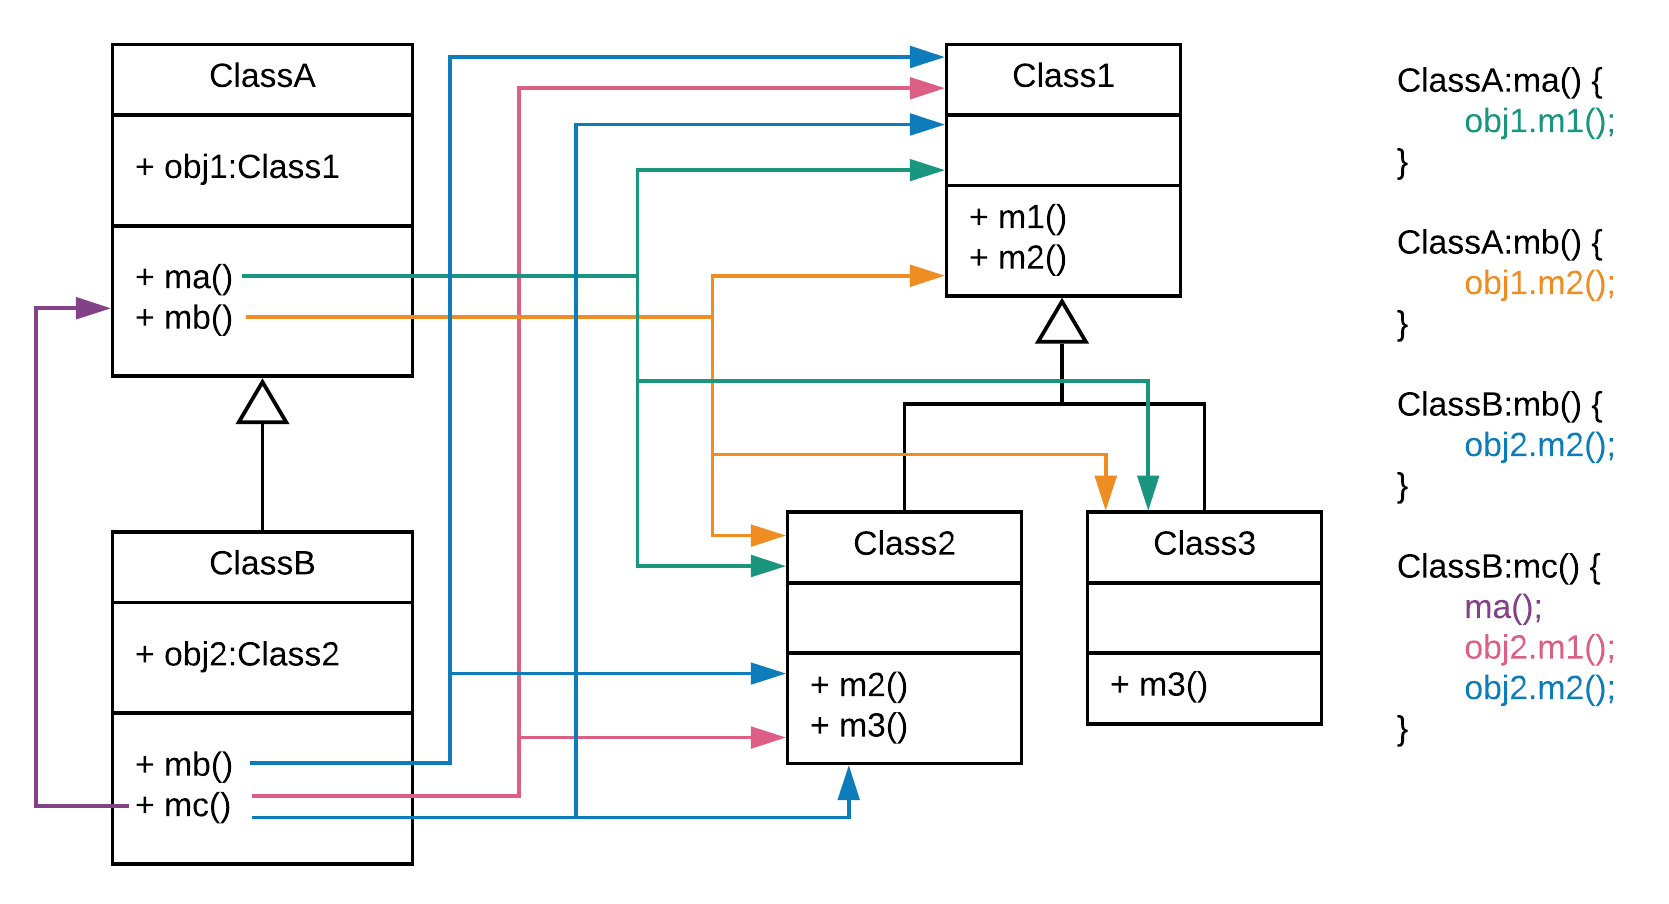
\includegraphics[height=4.4cm]{img/specialcases.png}
\caption{Example of coupling special cases, based on example from Briand et al. \cite{briand1999unified}}
\label{fig:specialcases}
\end{center}
\end{figure}

In order to answer the first question, we focus on the method \texttt{mc} of \texttt{ClassB} in Figure \ref{fig:specialcases}. This method invokes \texttt{ma} of \texttt{ClassA}, a class from which \texttt{ClassB} inherits. This is known as inheritance-based coupling and has been considered a special case of coupling in some studies. Should this connection be considered as a special case and be counted separately from the rest when considering maintenance effort? If there is a change in an inherited method that a class is using, it will require the same maintenance effort than in the case the method is not inherited. Therefore, our metrics \textbf{include inheritance-based coupling without distinction}.

Next, we discuss about whether to account for polymorphism. In this case we look at the methods of \texttt{ClassA}. This class contains an attribute of type \texttt{Class1}, which considering dynamic assignation of types could also be of type \texttt{Class2} or \texttt{Class3}. In this case, we have do consider if a call to a method of \texttt{Class1} would create coupling with \texttt{Class2} and \texttt{Class3}, and if it makes a different if the method is overridden or not. First, the method \texttt{ma} invokes \texttt{m1}, which is not overridden by any of the descendants of \texttt{Class1}. In this case, if there is a change in \texttt{Class2} or \texttt{Class3} it will not require changes in this call, since the invoked method stays the same. In contrast, method \texttt{mb} calls \texttt{m2}, which is overridden in \texttt{Class2}. Here, the implementation of \texttt{m2} in \texttt{Class2} could be updated, and this may affect the way \texttt{ClassA} uses it, and therefore changes may be needed. Thus, we consider that it is necessary to \textbf{account for polymorphism}.

Lastly, we discuss about how do decide if a method belongs or not to a class. We have two options: A method belongs to the class that implements it (could be more than one since we account for polymorphism), or a method belongs to the class that it is referenced from. An example of this can be found in the last two lines of the method \texttt{mc} of \texttt{ClassB}, which call method \texttt{m1} and \texttt{m2} on an object of type \texttt{Class2}. The difference is that \texttt{m1} is implemented in \texttt{Class1} and \texttt{m2} is overridden in \texttt{Class2}. From a maintenance perspective, if the method \texttt{m1} is updated in \texttt{Class1}, this will probably require updates in \texttt{ClassB} as well. However, changes in \texttt{Class2} will not generate a need to update the method call in \texttt{ClassB}. In addition, if  \texttt{m2} is updated in \texttt{Class1}, it will not make a difference for this call of \texttt{m2} since it is not executing the implementation of \texttt{Class1}. Therefore, \textbf{a method call creates coupling with the class that contains the implementation}.

\section{Formal definition of the metrics}
Based on the characteristics of coupling described in the previous section, we define two coupling metrics. The difference between these metrics is the type of connection measured.

\subsection{Metric 1: Method invocation coupling}
This metric measures the dependency between two libraries, one acting as client ($L_c$) and the other as server ($L_s$), based on the method invocations from $L_c$ to $L_s$. Based on the criterion 3 discussed in the previous section, this metric is calculated for each of the classes implemented in $L_c$, and for each of the methods implemented in these classes. For eacn one of the implemented methods in $L_c$ ($M(L_c)$), we count the number of individual invocations to a method of $L_s$ ($nII(m_c,L_s)$). For each method invocation made by the methods implemented in $L_c$, we count only the ones that are implemented in stable classes (not implemented in $L_c$). The set of stable methods invoked is $SIM(m_c)$.

Then, according to criterion 6, it is necessary to take into account all the polymorphic implementations of the invoked method that are implemented in $L_s$. Therefore, we intersect the set of polimorphic implementations of an invoked method ($PM(m_s)$) with the set of methods implemented in $L_s$ ($M(L_s)$). Finally, to obtain the number of individual invocations, we multiply the number of times a method has been invoked ($nI(m_c, m_s)$) by the number of polymorphic implementations of the method in $L_s$ ($nP(m_s, L_s)$).

\begin{equation}
\verb|MIC|(L_c, L_s) = \sum_{m_c \in \verb|M|(L_c)} \verb|nII|(m_c, L_s)
\end{equation}

\begin{equation}
%\begin{aligned}
   \verb|nII|(m_c, L_s) = \sum_{m_s \in \verb|SIM|(m_c)} \verb|nI|(m_c, m_s)*\verb|nP|(m_s, L_s)
%\end{aligned}
\end{equation}

\begin{equation}
    \verb|nP|(m_s, L_s) = |\verb|PM|(m_s) \cap \verb|M|(L_s)|
\end{equation}

\subsection{Metric 2: Aggregation coupling}
The process for this metric is similar to the one of the first metric. However, in this case, the metric counts the number of times in which a class of $L_c$ has an attribute which type is a class implemented in $L_s$. Therefore, the metric will be calculated for each class implemented in $L_c$ ($C(L_c)$). For each class, we consider only those attributes types that are stable classes (not implemented in $L_c$). The set of attribute types in a class that are stable is $SAT(c_c)$.

According to criterion 6, in this case, to account for polymorphism we count all the descendants of the class that are implemented in $L_s$. Therefore, we intersect the set with the descendants of the class ($DC(c_s)$) with the set of classes implemented in $L_s$ ($C(L_s)$). Finally, to count individual connections, we multiply the number of times a the client class has an attribute of type the server class ($NA(c_c, c_s)$) by the number of descendants of the class (class included) implemented in $L_s$ ($nDC(c_s,L_s)$).

\begin{equation}
  \verb|AC|(L_c,L_s) = \sum_{c_c \in \verb|C|(L_c)} \sum_{c_s \in \verb|SAT|(c_c)} \verb|NA|(c_c, c_s)*\verb|nDC|(c_s, L_s)
\end{equation}

\begin{equation}
    \verb|nDC|(c_s, L_s) = |\verb|DC|(c_s) \cap \verb|C|(L_s)|
\end{equation}

\section{Preliminary Results}



\section{Conclusion and Next Steps}
With this initial work on the research, we have defined the first two metrics to measure the degree of library dependency. To do so, we have used the framework defined by Briand et al. to formulate the definition of coupling to be measured. The framework has been extended to adapt it to the use case of dependencies between libraries. The result is the definition of two metrics which measure different types of connection between libraries: method invocations and aggregation.


\subsection{Next Steps}
The following step, will be to define the metrics to measure transitive dependencies. Then, we will perform the theoretical validation of the metrics. This will be done by validating that the proposed metrics fulfill certain properties. For example, Briand et al. \cite{briand1999unified} define five properties of the coupling metrics. Besides, the applicable subset of the set of metrics defined by Meneely et al. \cite{meneely2013validating} will also be validated.

Another part of the work will involve implementing a proof of concept tool (PoC) to calculate the metrics. The PoC will be done by using versioned call-level graphs, to obtain a result as precise and fine-grained as possible.
Once the PoC is working and it has been used with a relevant set of libraries, we will evaluate the results. Various types of evaluations will be conducted: First, evaluation of the PoC itself, by analyzing the runtime complexity of the implementation. Then, the metrics will be compared in order to determine the correlation between these. In addition, some experiments will be conducted, comparing the effort invested in updating and maintaining a dependency with the associated coupling.

Then, the work will be focused on the second research question. First, we will study the different cases of dependency replacement and how each of these cases may affect a project. Then, for each case, we will determine how it affects the code. Besides, we will research the applicable methods to calculate the needed effort to implement the replacement of the dependency. Finally, we will validate the proposed method by comparing the real effort invested in a replacement with the effort estimated by our model.

\bibliographystyle{alpha}
\bibliography{res}
%inline the .bbl file directly for mailing to authors.

\end{document}
